\documentclass{article}
\usepackage{graphics}
\usepackage{graphicx}
\usepackage{tabularx}
\usepackage[titletoc,title]{appendix}

\title{SBS trigger and electronics update}

\author{A. Camsonne, M. K. Jones}

\begin{document}
\maketitle
\section{Experiment overview}

\section{Electronics inventory}

\subsection{Pipelined electronics}
\subsubsection{JLab Flash ADC 250}
The JLab Flash ADC 250 is a VME 12 bit 250 MHZ Flash ADC with 16 channels. It can transfer data through the VME64X backplane in 2eSST protocol which can reach up to 200 MB/s, it can also transfer data through the VXS backplane which is serial multiline point to point protocol with data transfer up to 8 GBit/s per lane. Each FADC has 4 VXS lanes. It has 8 microsecond pipeline. It will be used for the Hadron Calorimeter readout to allow to produce a HCAL trigger by doing clustering of the FADC data in a dedicated logic module the VXS Trigger Processor (VTP).  
\subsubsection{F1 TDC}
The JLAB F1 TDC is base on the F1 chip, it is a pipelined multihit pipelined TDC with 64 channels in low resolution mode 120 ps and 32 channel in high resolution mode of 60ps. It can be readout using the VME backplane also using the 2eSST transfer protocol for data rates up to 200 MB/s. It will be used for Neutron Form Factor experiment where the neutron momentum is measured by time of flight. The F1 TDC will supplement the FADC which typically can give a timing resolution of 0.3 ns.
\subsubsection{SubSystem Processor}
The SubSystem Processor is part of the standard JLAB pipeline electronics system. It is a VME64X board with 8 QSFP optical port with VME 2eSST capability (200 MB/s) and VXS connectivity.
The initial goal of the SSP was to gather data from different crates of FADC to concentrate the data to a single logic module Global Trigger Processor (GTP) which is superseded by the VXS Trigger Processor (VTP). Each optical link can transfer up 6.25 Gb/s giving a 25 GBit/s bandwidth for each QSFP connector the board can send data to the VTP using up to 4 VXS lines with each line having a 6.25 Gbit/s bandwith.
Since this module is capable of reading a lot of data in parallel it will also be used to readout the GEM electronics using their optical cable.
\subsubsection{VETROC}
The VXS Electron Trigger Read Out Controller (VETROC) is a board to generate an electron trigger from a silicton strip detector. It was designed as a flexible 192 channels pipelined input output/register compatible with JLAB pipeline electornics system. It allows to have the status of each of its input at 250 MHz sampling which can be used for trigger purpose in conjunction with the FADC data.

\subsubsection{VXS Trigger Processor}
The JLAB pipeline system relies on the VXS bus to transfer the FADC data to a central module called General Trigger Processor (GTP) where the logic involving all the FADC channels can be processed. A new version of this module with additionnal optical link on the front panel and VXS lines on the back was designed and called VXS Trigger Processor (VTP).


\subsection{Fastbus electronics}
\subsubsection{Lecroy 1881M ADC}
The electromagnetic calorimeter having a large number of channel will be readout using the Fastbus 1881M.
It is a high Density, 64 Channels Per FASTBUS Slot 13 bit integrating ADC. It has a conversion Time of 12 µsec in 13-Bit Mode (9 µsec in 12-Bit Mode) a fast clear is possible to allow a L1 L2 logic reducing the dead time due to conversion. It can be programmed to perform online pedestal suppression. It has a buffer up 64 Events.
Theoretical data transfer is up to 40 MB/s with an actual sustained rate of 15 MB/s.
A fast clear can be issued and the module is ready to register another trigger after 1 $\mu$s.

\subsubsection{Lecroy 1877S TDC}
All other hit based detectors (CDET, GRINCH) will be read with Fastubs 1877S Multihit Time-to-Digital Converter with Data Supression.It is a  High Density, 96 Channels Per FASTBUS Slotwith 0.5 ns resolution.
It is a multhit TDC with up to 16 Hits/Channel and it can detect rising and/or falling edge which will allow to measure the amplitude of the signal with time over threshold information. It can hold up to 8 events in its buffer. The module can defineBuilt-in Data Zero Suppression, Data Compression and Data Compaction
    Multiple Event Buffer, 8 Events
    Fast clear after 1 $\mu$s 300 ns after.

\section {Proton Form Factor}

\subsubsection{ECAL trigger}
 \label{sec:ecal-trig}
 In Fig.~\ref{fig:ECALTrig}, the left plot shows the distribution of events at the front of the ECal
 and overlayed on the individual blocks. The middle plot shows the groups of 2x4 blocks ( outlined in red)
 which will go into the sum of 8 modules. Around the edges the groups include less than 8 blocks 
 (outlined in green). There are a total of 219 sum of 8 modules needed.
 The sum of 8 modules pass the individual analog signal of each block to a connector in the
 back of the module. A cable goes from this connector goes to a nearby patch panel on the ECal platform. The patch panel goes to a long 500ns delay cable which brings the signal to
 another patch panel in the electronics hut. This patch panel changes from the individual BNC cables into a 16 channel ribbon cable which goes into the 1881M ADC. 
 Table~\ref{tab:ECALadctime} gives the total propagation time of the individual signal from each block along with the breakdown into the different components.
 \begin{table}[b]
 	\begin{tabular}{|l|l|} \hline
 		Cable length from PMT to sum of 8 module & 40ns \\ \hline
 		Sum of 8 module transit time & 10ns \\ \hline
 		Cable from back of the Sum of 8 module to patch panel on ECal & 6ns \\ \hline
 		Cable from ECal patch panel to patch panel in electronics hut & 500ns \\ \hline
 		Ribbon Cable from patch panel on ECal & 15ns \\ \hline
 		  		Total time & 571ns \\ \hline  		   		  		 		 
 	\end{tabular}
 	\caption{The contributions to total propagation time  of the ECal calorimeter signals.}
 	\label{tab:ECALadctime}
 \end{table}
 
 
 
 For the formation of the trigger, the sum of 8 modules have 6 outputs of the summed signal.
 In the right plot of Fig.~\ref{fig:ECALTrig}, the groups of 32 blocks which sum 4 groups of
 8 blocks are indicated by purple filled circles at the intersection of 4 groups of 8. 
 The group of 32 blocks overlap
 by two groups of 8 in both horizontal and vertical directions. So most of the
 groups of 8 have to go to 4 groups of 32. At the edges the groups of 8 feed into
 two groups of 32. There are 192  groups of 32. The output of the groups of 32 would go into 16 channel
 discriminators. A total of twelve 16-channel discriminators would be needed. The  outputs of the
 discriminator would go into a 16-channel mixed logic unit to produce an "OR" for each set of
 16 inputs. The 12 "OR" signals would go into a final 16-channel mixed logic unit to 
 a trigger that needs to be sent to the Trigger Supervisor as the Level One trigger. A 50m fast R8 cable will bring the trigger from the ECal platform to the Trigger Supervisor
 which will be located in a VXS crate in the electronics hut. The Trigger Supervisor
 takes 40ns to produce the ADC gate and the cable from the Trigger Supervisor to the
 trigger distribution card in the back of the FASTBUS crate takes 25ns. The total time
 is 391ns which is 180ns less than the 571ns for the propagation time of the individual
 signals to the ADC.
 
 \begin{table}
 	\begin{tabular}{|l|l|} \hline
 		Cable length from PMT to sum of 8 module & 40ns \\ \hline
 		Sum of 8 module transit time & 10ns \\ \hline
 		Cable from Sum of 8 module to FI/FO for group of 32 & 24ns \\ \hline
 		FI/FO module transit time & 10ns \\ \hline
 		Cable from FI/FO to the 16 channel discriminator & 4ns \\ \hline
 		 16 channel discriminator  transit time & 10ns \\ \hline
 		 Cable from the 16 channel discriminator to 16 channel mixed logic unit& 4ns \\ \hline
  		 16 channel mixed logic unit  transit time & 10ns \\ \hline
  		 Cable from the 16 channel mixed logic units to final 16 channel mixed logic unit& 4ns \\ \hline
  		 16 channel mixed logic unit  transit time & 10ns \\ \hline
  		 50M fast cable from the ECal platform to Trigger Supervisor & 200ns \\ \hline
  		 Transit time in TS to produce the ADC gate & 40ns \\ \hline
  		 Cable from TS to logic fan  & 6ns \\ \hline\hline
                 Logic fan  & 10ns \\ \hline\hline
                 Logic fan to FASTBUS crate & 25ns \\ \hline\hline
  		 Total time & 407 ns \\ \hline  		   		  		 		 
 	\end{tabular}
 	\caption{The contributions to total time formation of the ECal Level One trigger sued as the ADC gate.}
 	\label{tab:ECALTrigtime}
 \end{table}
 
 
 \begin{figure}
 	\centering
 	% Requires \usepackage{graphicx}
 	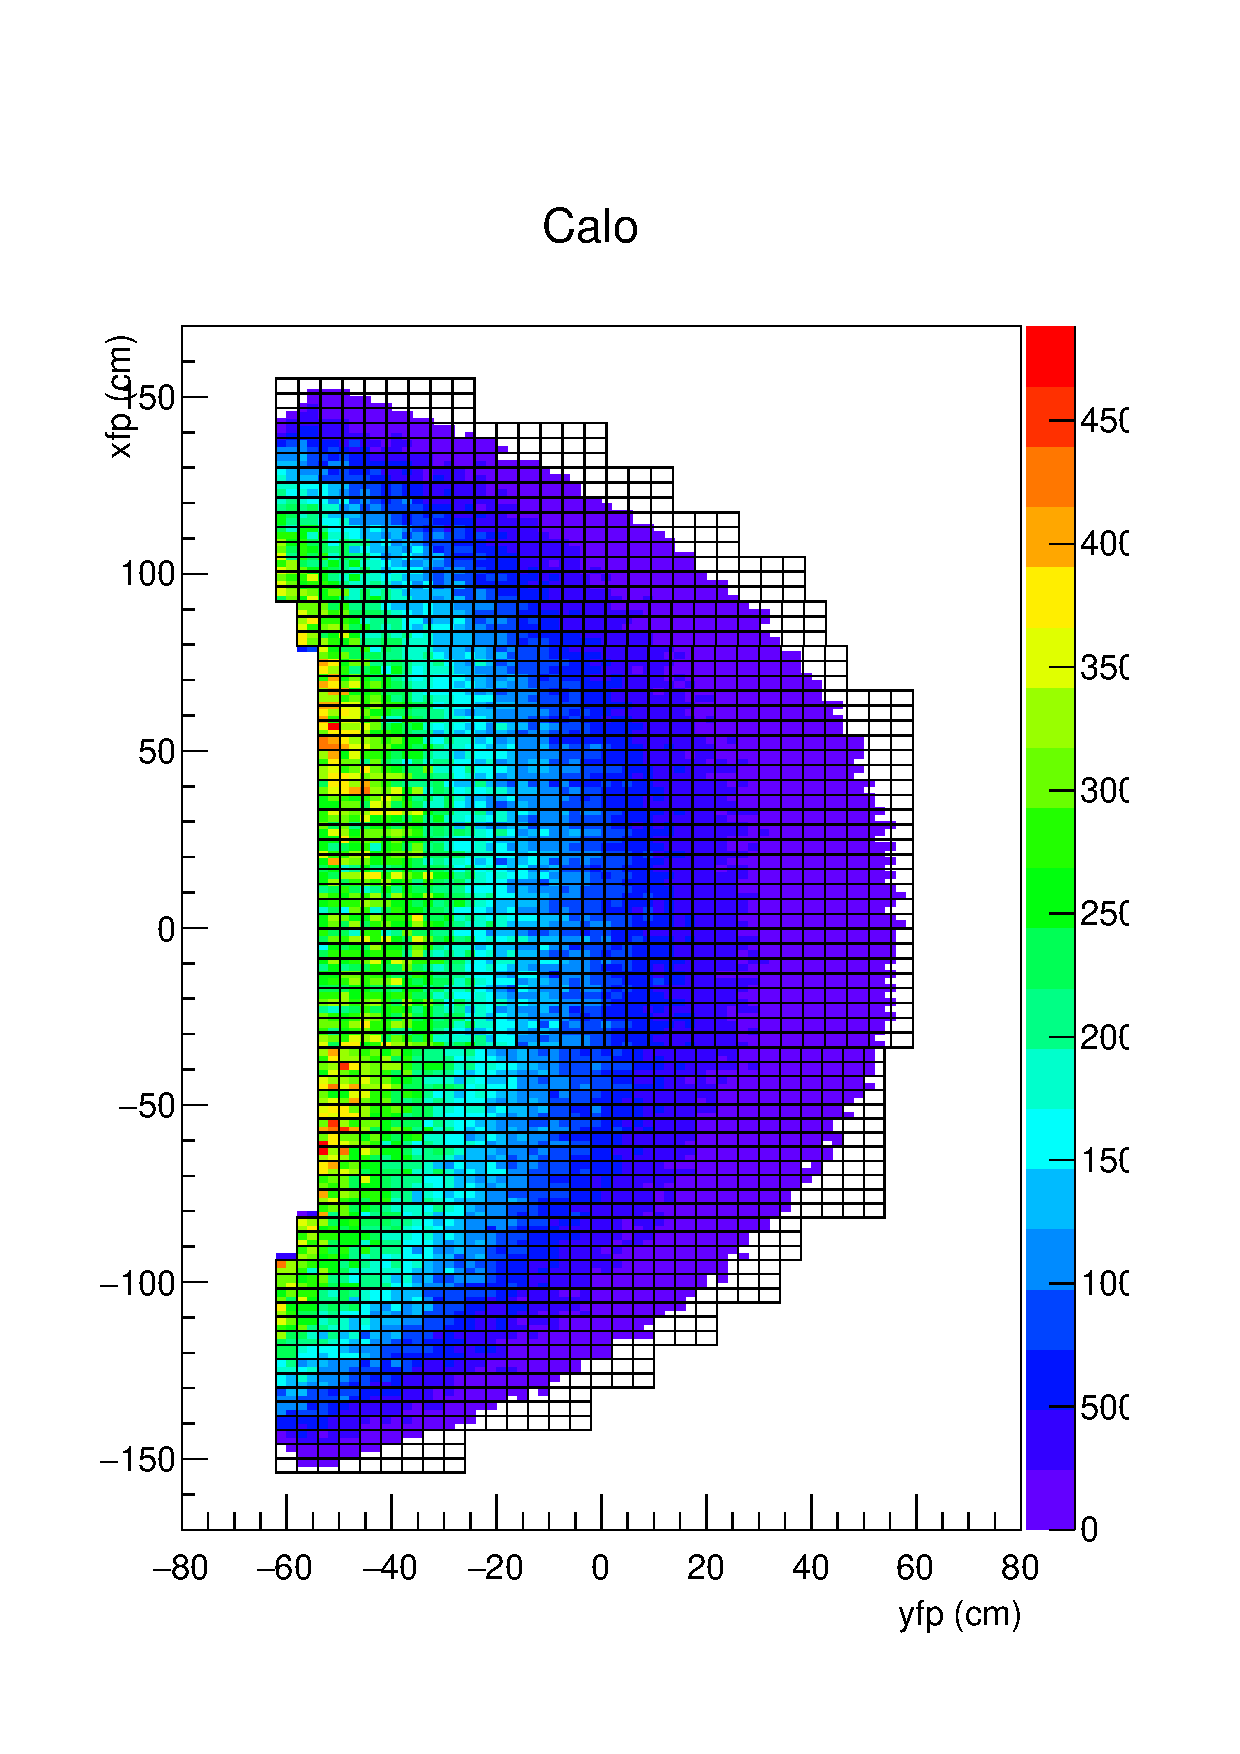
\includegraphics[width=0.3\textwidth]{cfpbox.pdf}
 	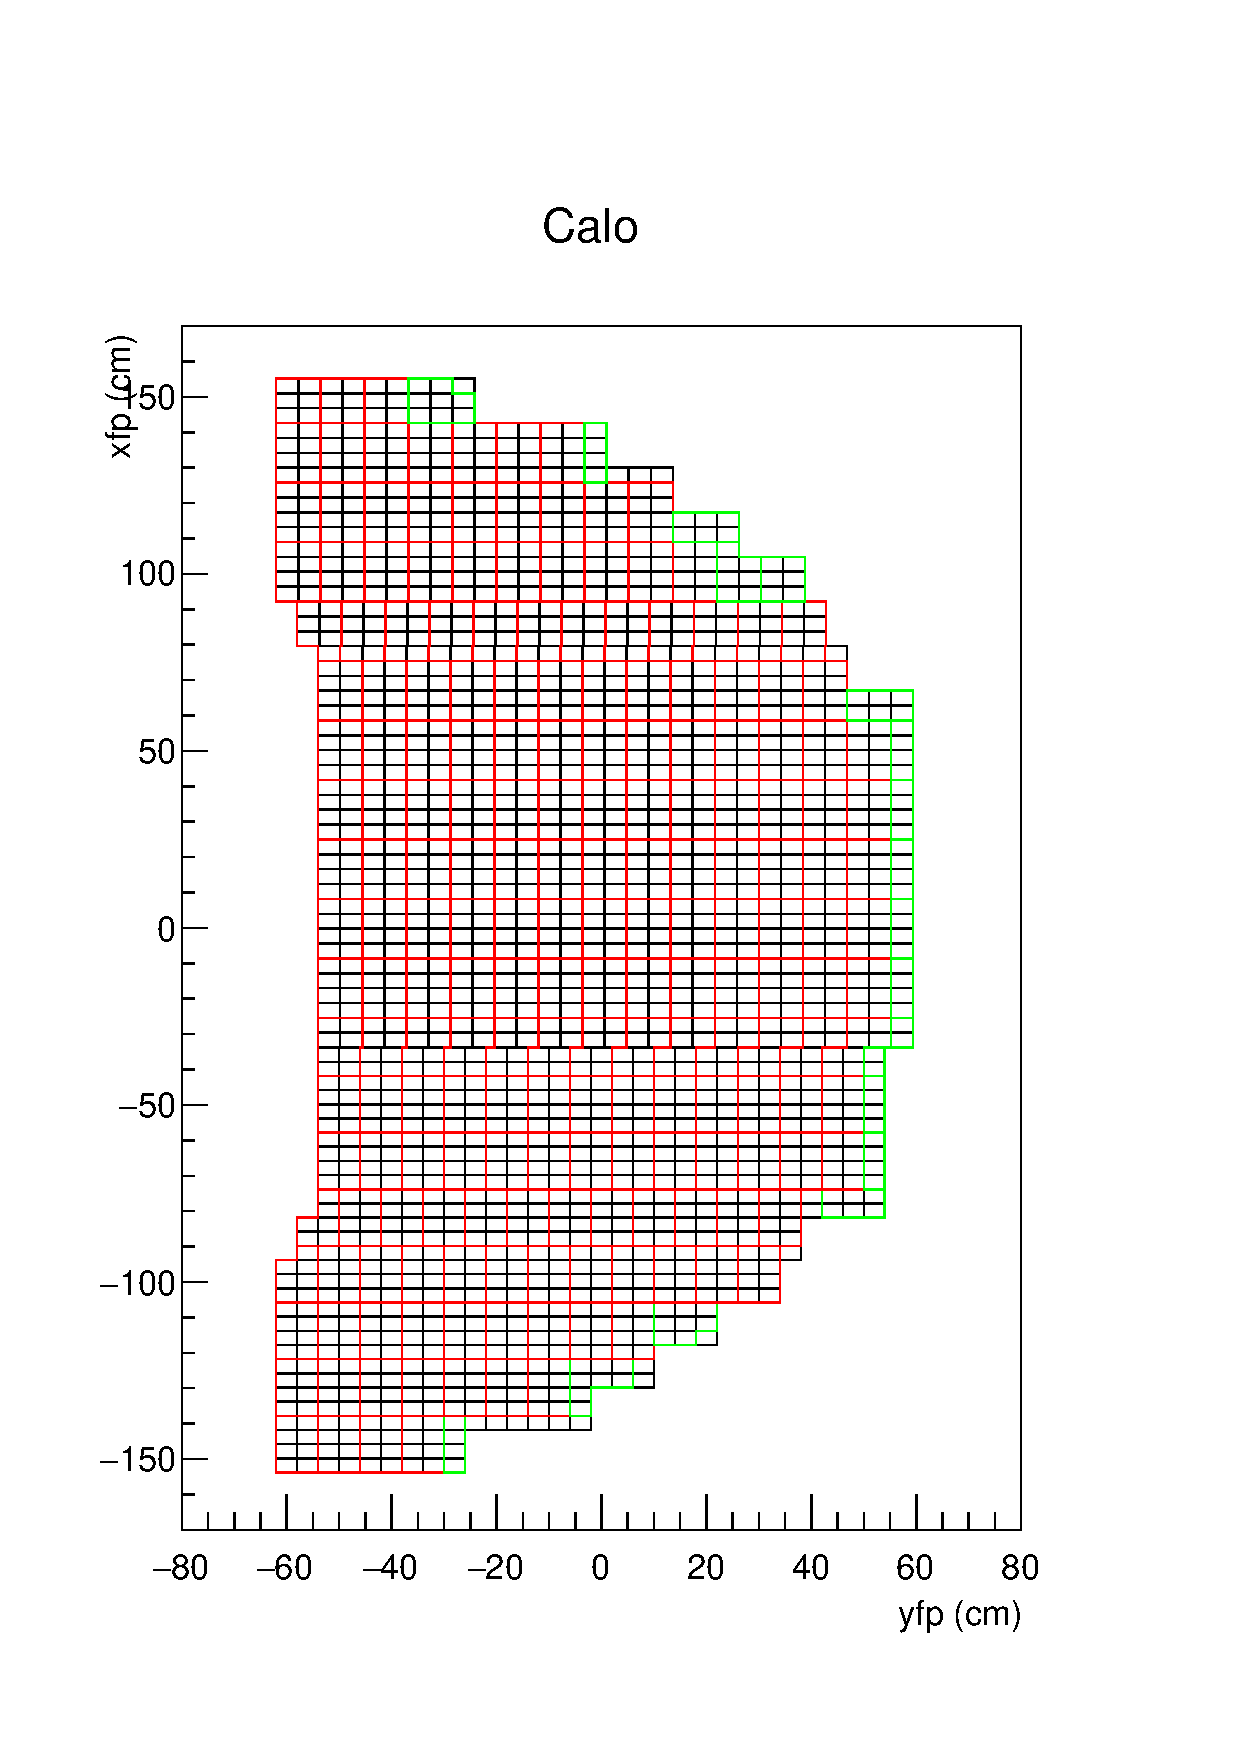
\includegraphics[width=0.3\textwidth]{cfpc.pdf}
 	 	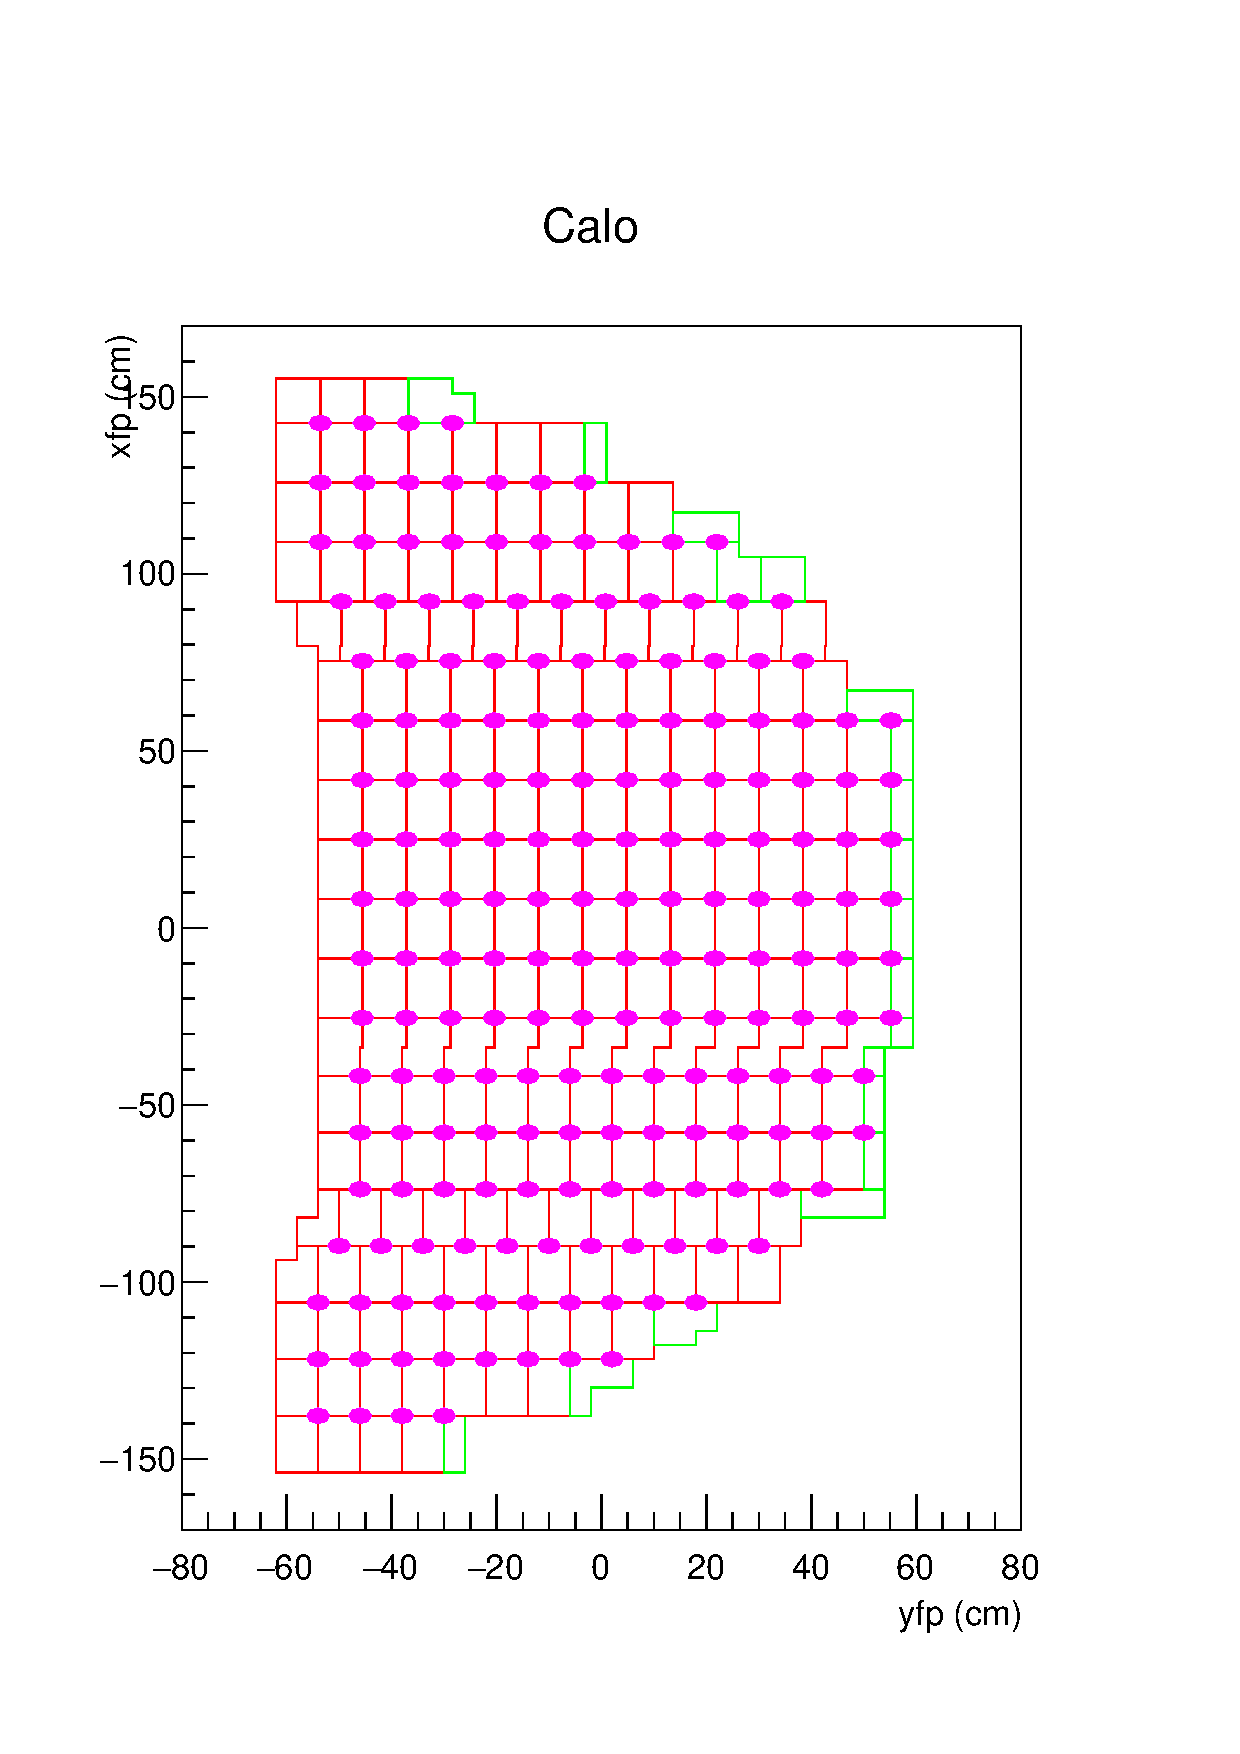
\includegraphics[width=0.3\textwidth]{cgr32.pdf}
 	 	\caption{The left plot is the distribution of elastic electrons in ECAL with the black rectangles representing
 		groups of 2x4 lead glass blocks. The right plot demonstrates
 		the scheme for make overlapping groups of 32 lead glass blocks to be used in the ECAL trigger with
 		details explained in text.  }\label{fig:ECALTrig}
 \end{figure}

\subsection{Hall layout}
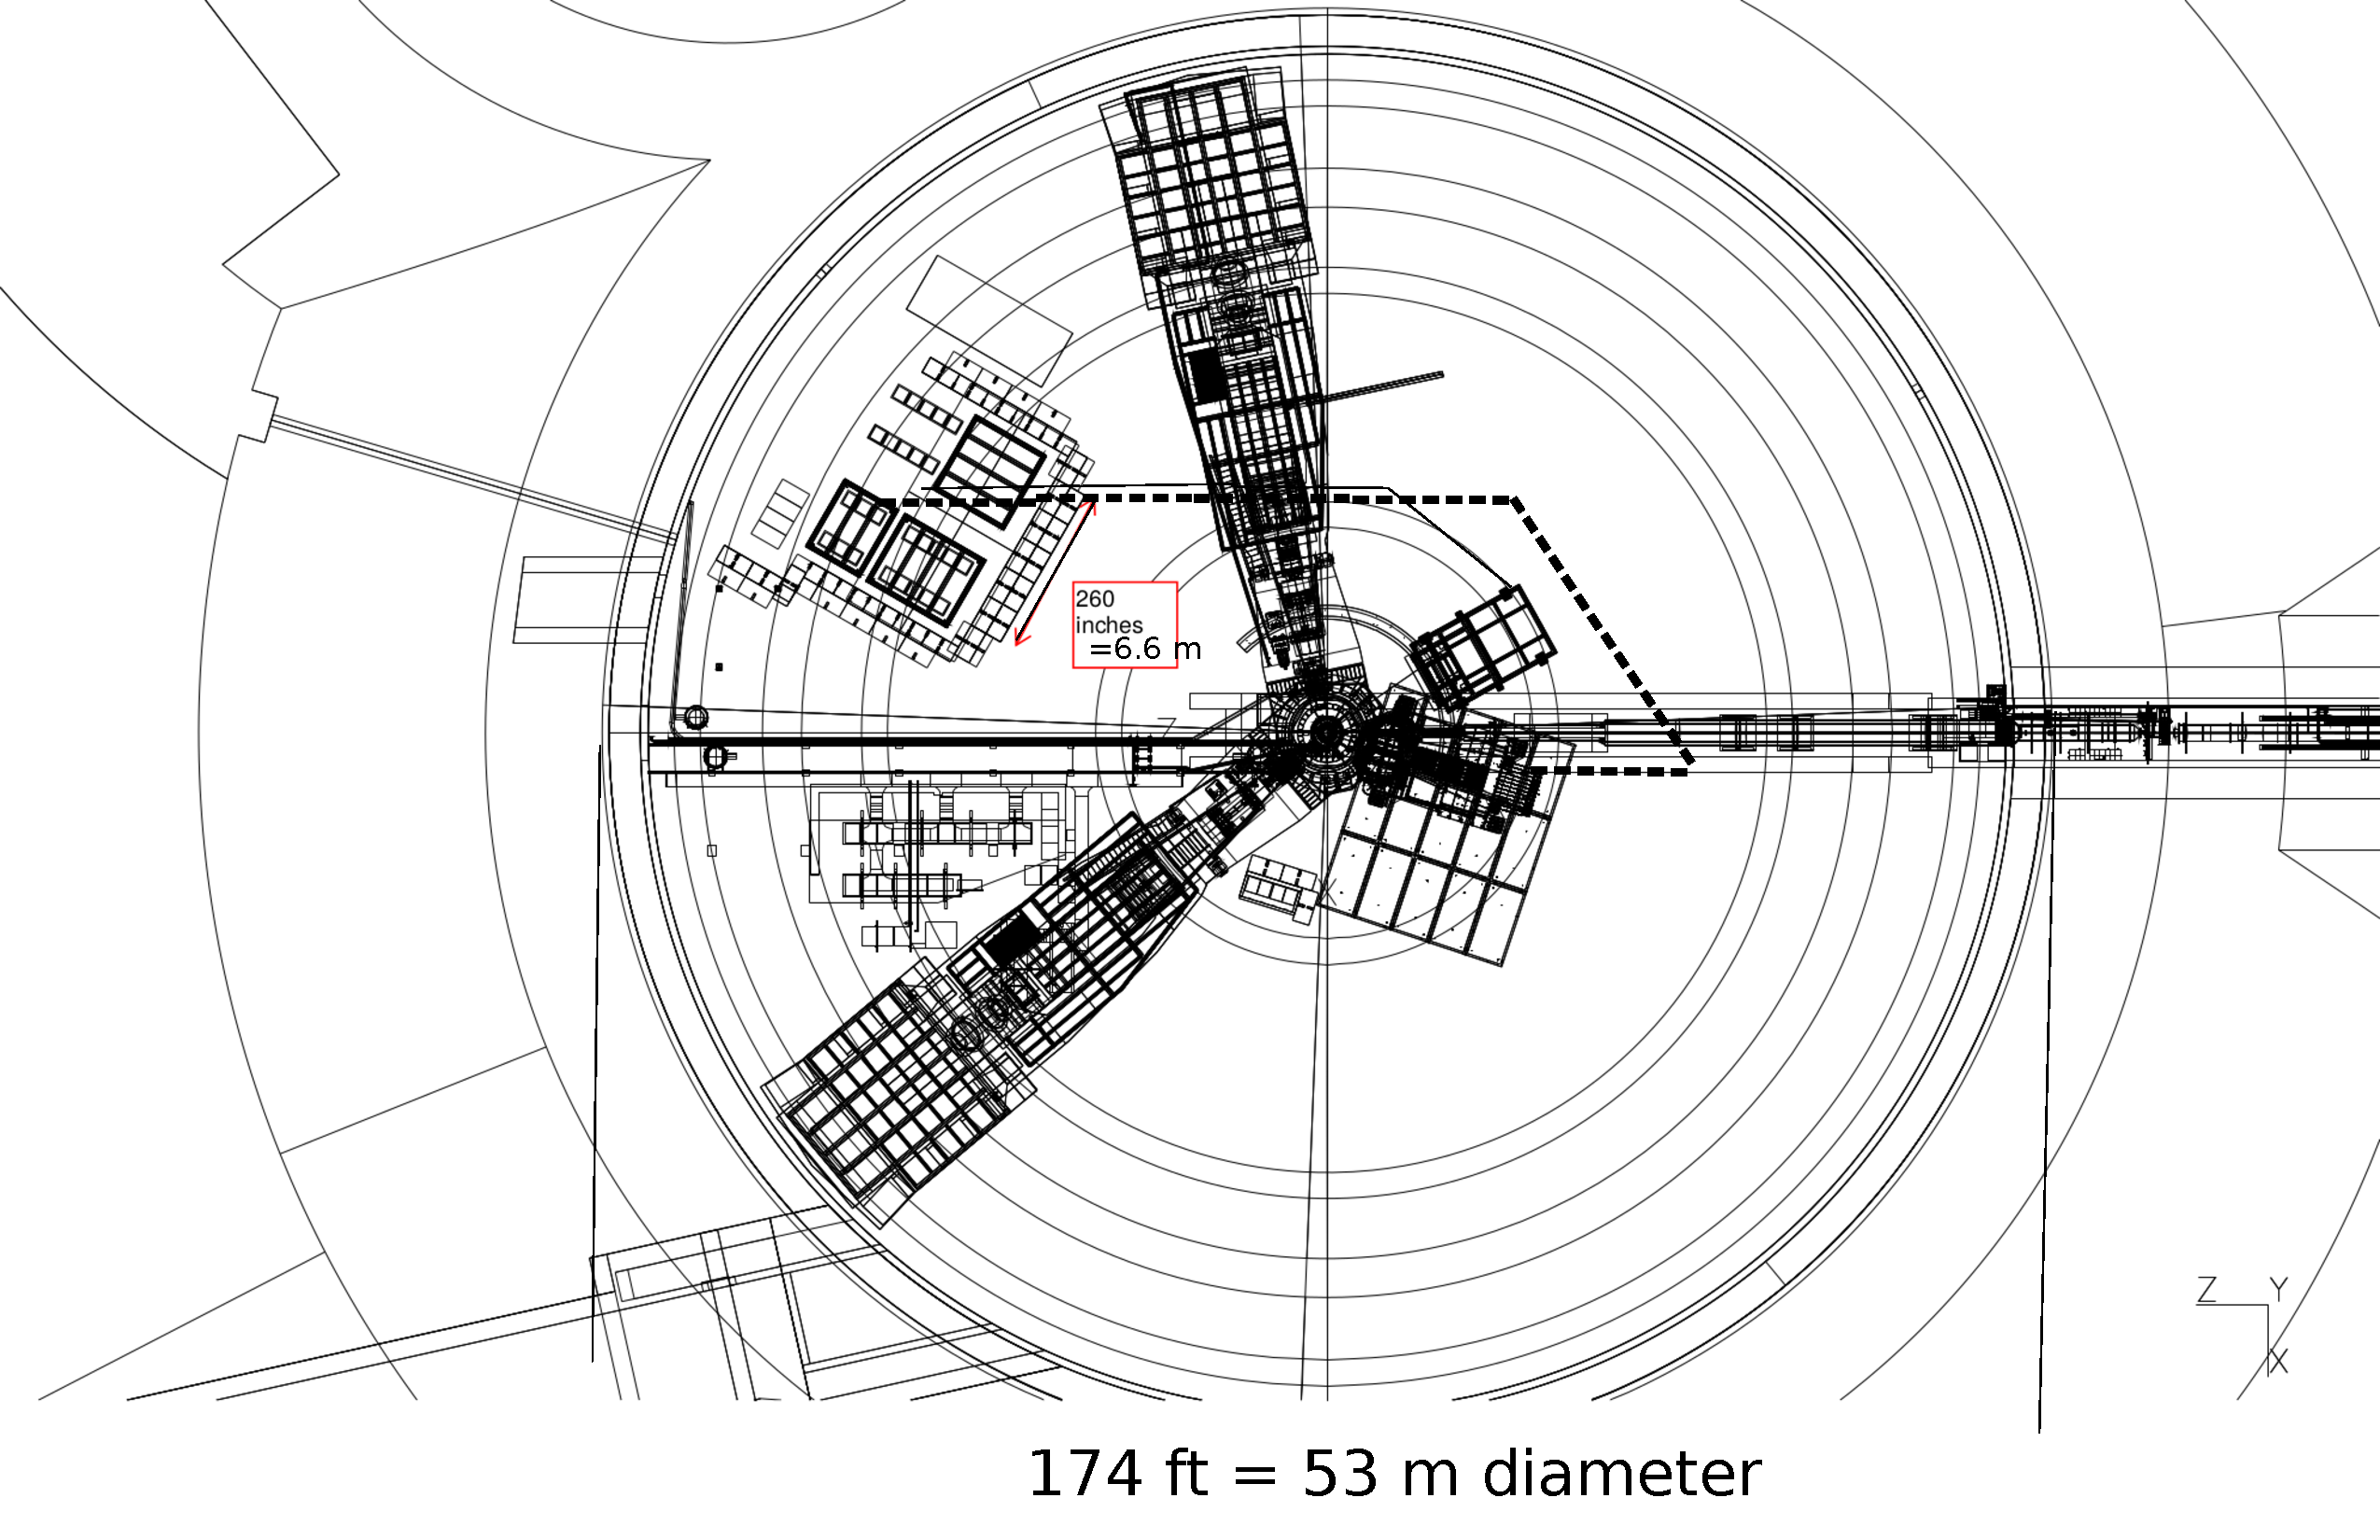
\includegraphics[scale=0.3]{figs/cablesHall.pdf}
 \subsection {Electronics layout}
 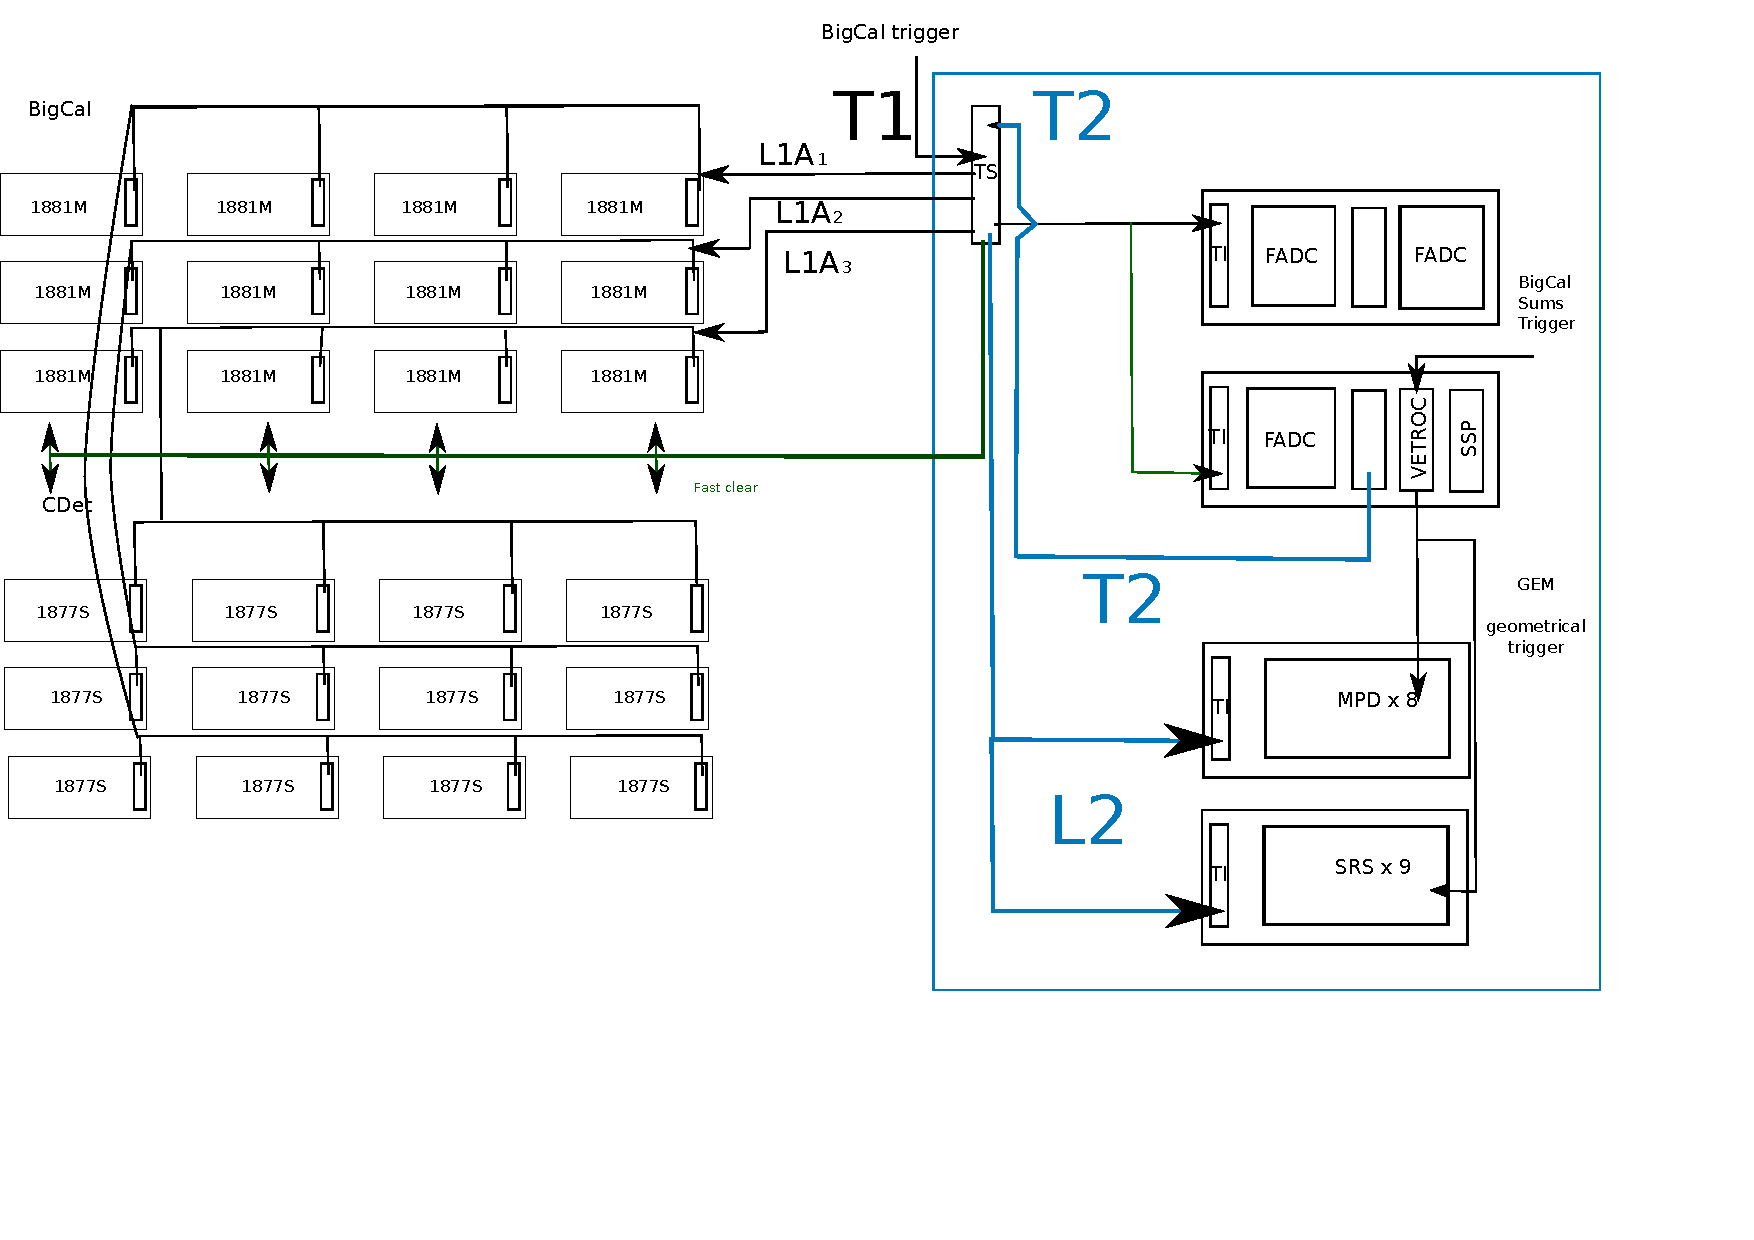
\includegraphics[scale=0.4]{figs/SBSlayout.pdf}

 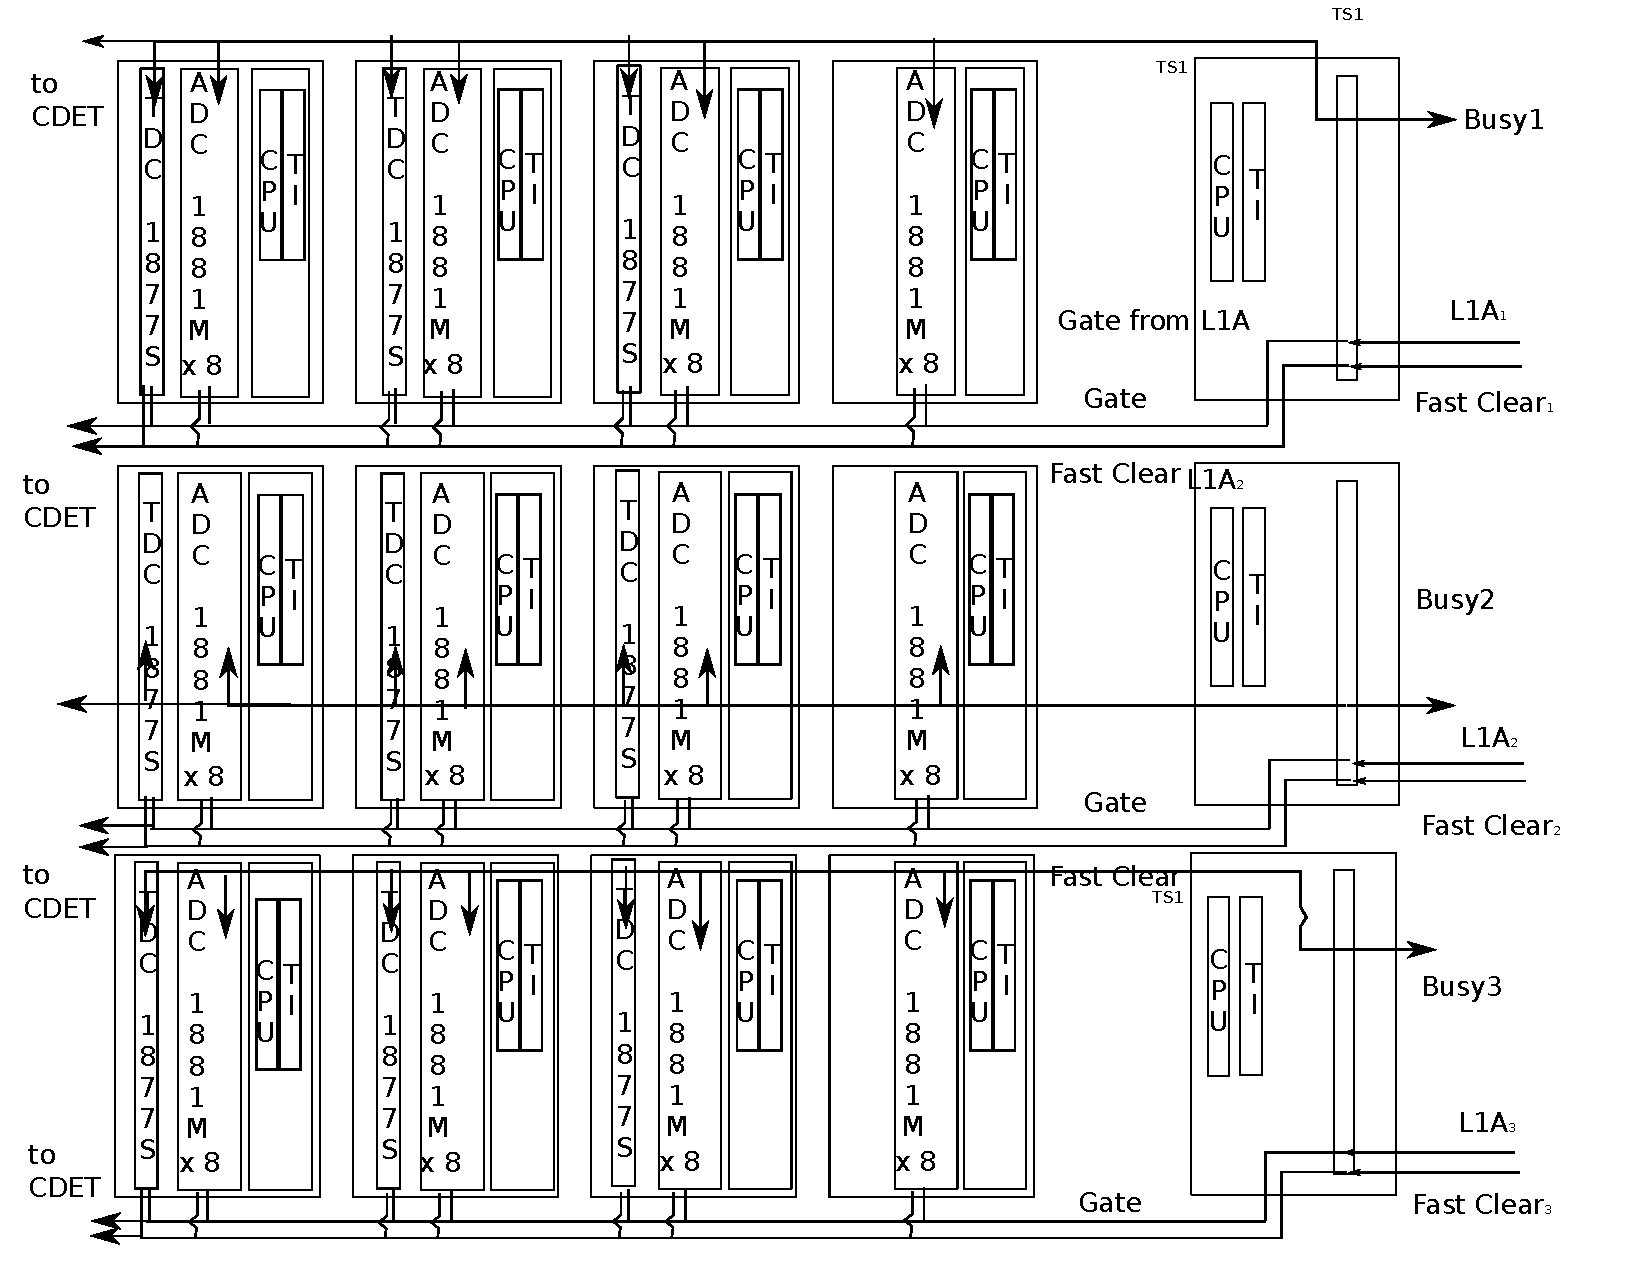
\includegraphics[scale=0.4]{figs/FastbusEcalDetailed.pdf}

\subsection{GEM readout}
 
 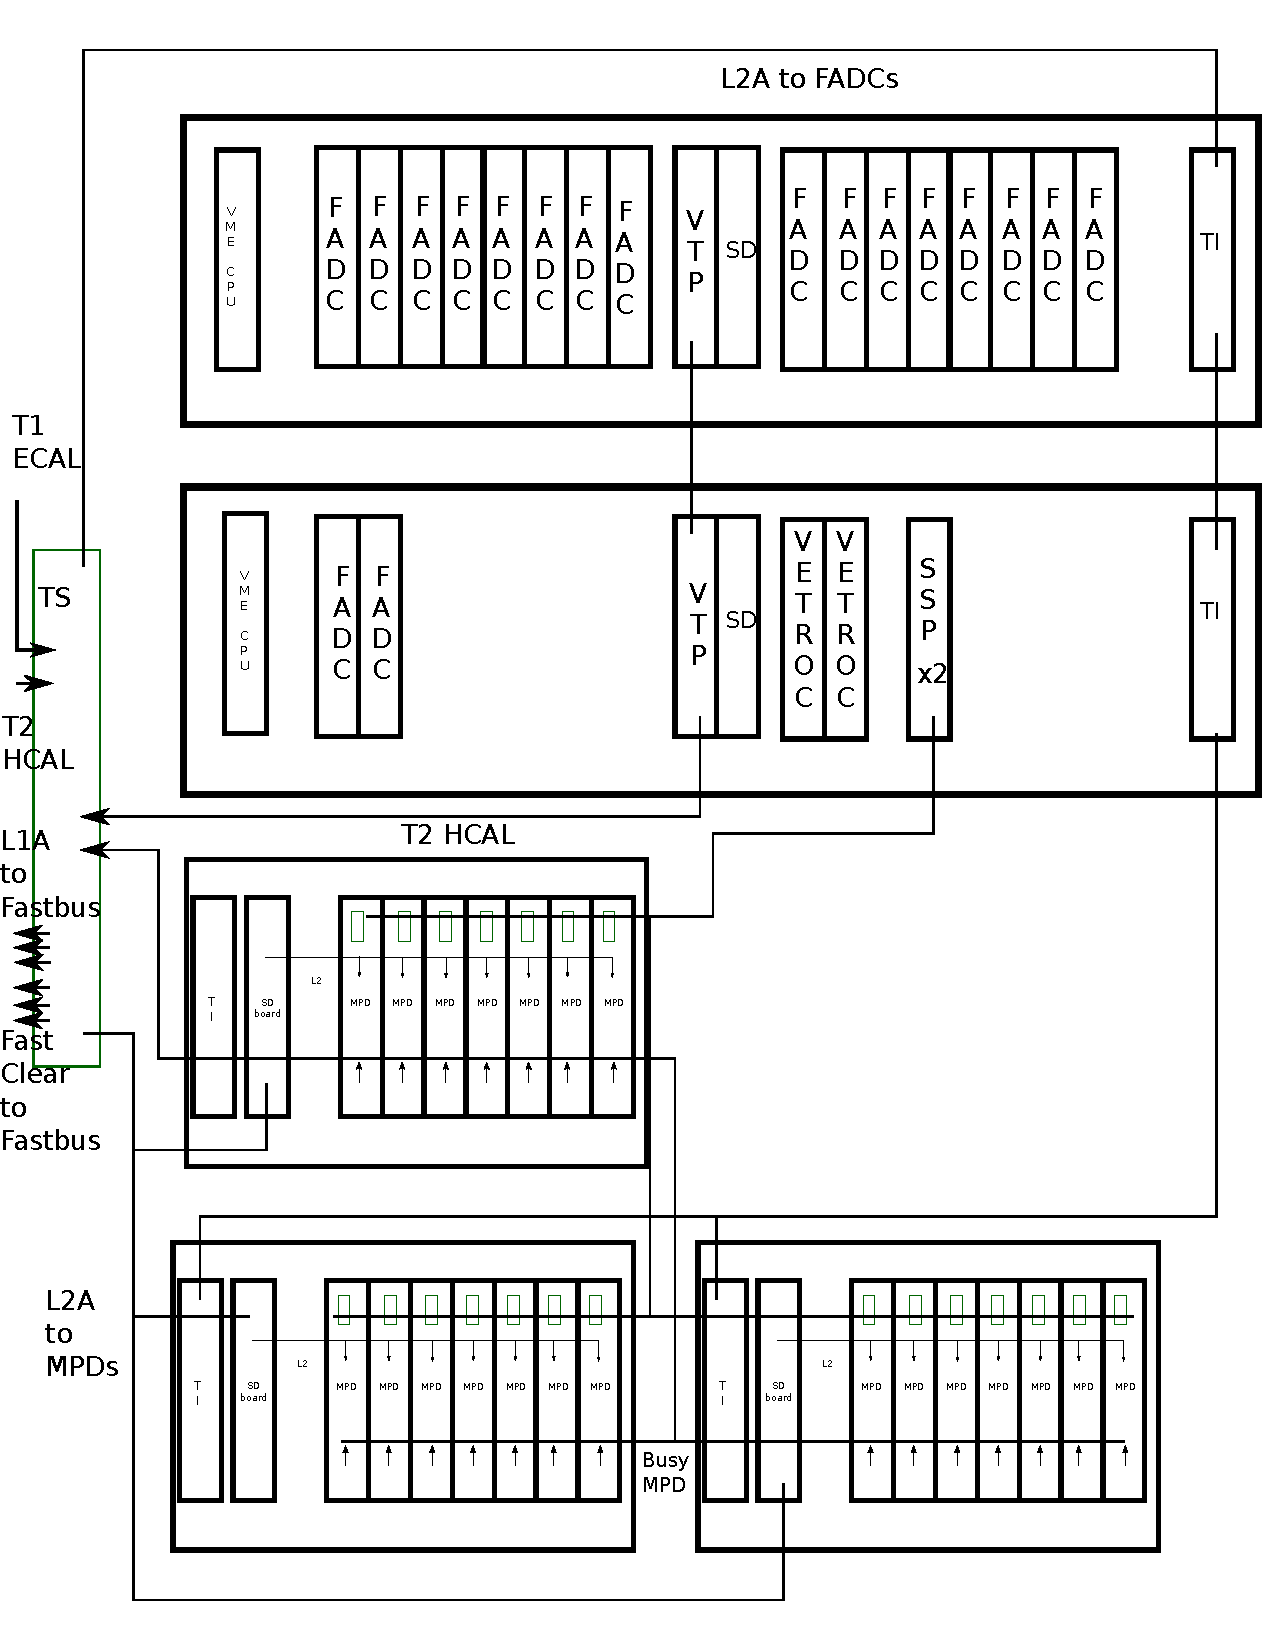
\includegraphics[scale=0.4]{figs/NewMPDDetailed.pdf}

  
 \subsection {Experiment timing}
 \newpage
	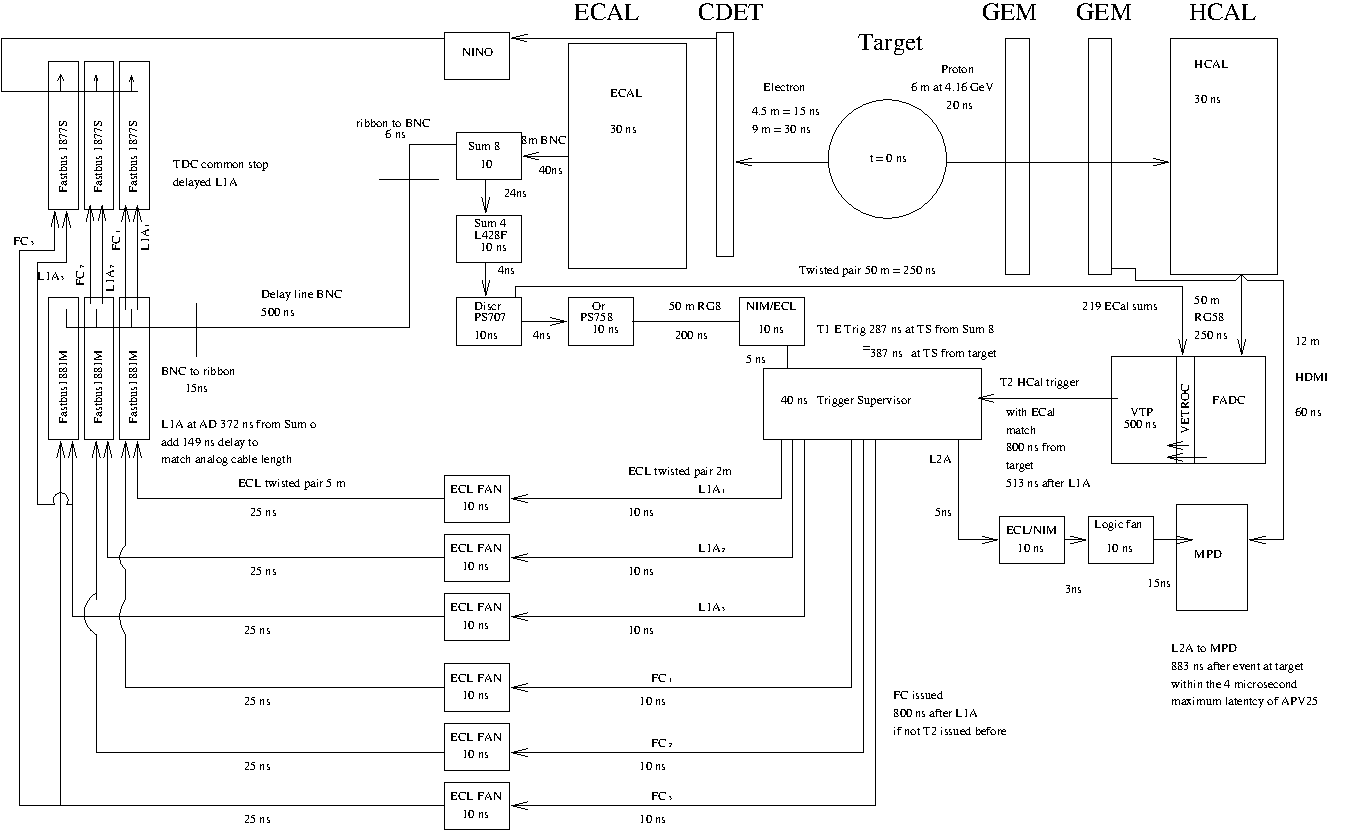
\includegraphics[scale=0.8,angle=90]{figs/GeP.pdf}

\subsection{Expected data rate}
        
\section {Neutron Form Factor experiments}
\subsection {The BigBite spectrometer}

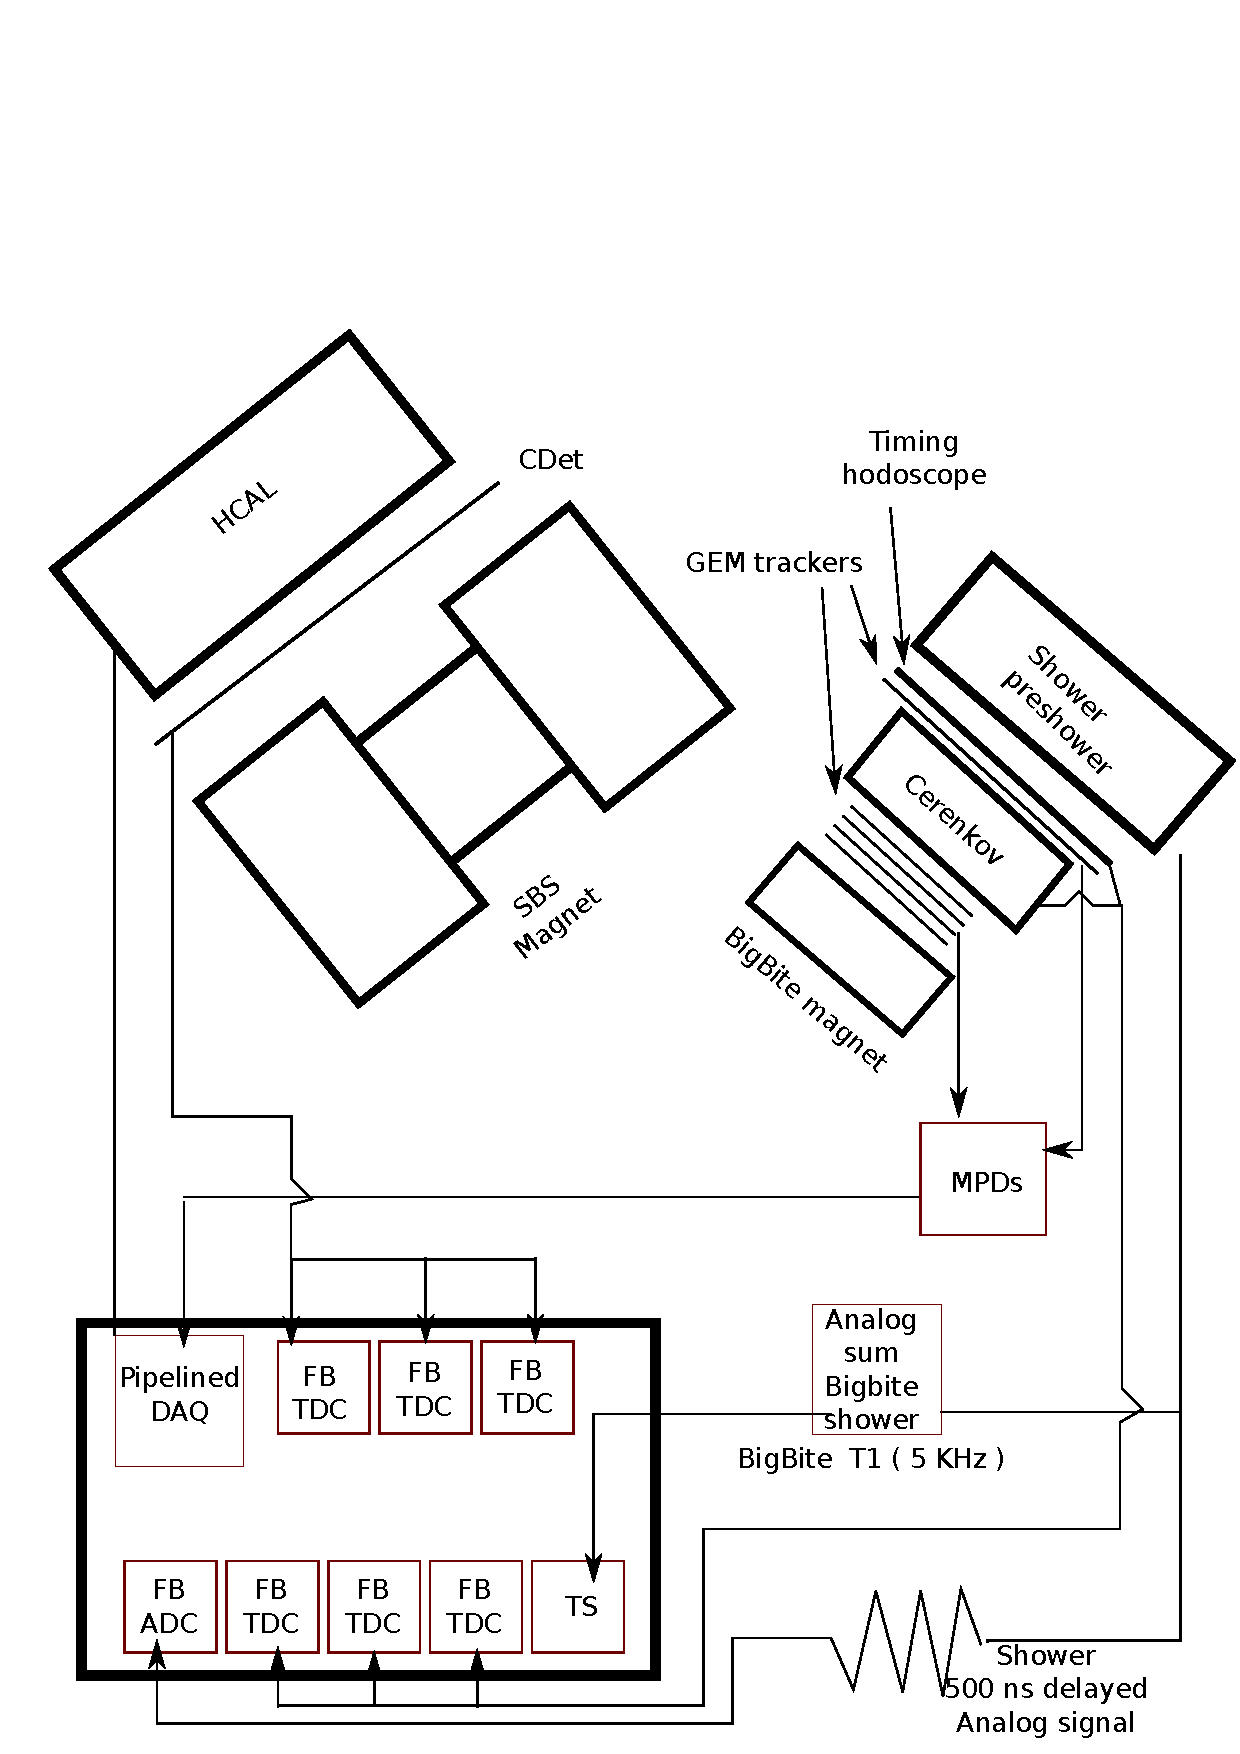
\includegraphics[width=0.8\textwidth]{figs/GeNlayout.pdf}

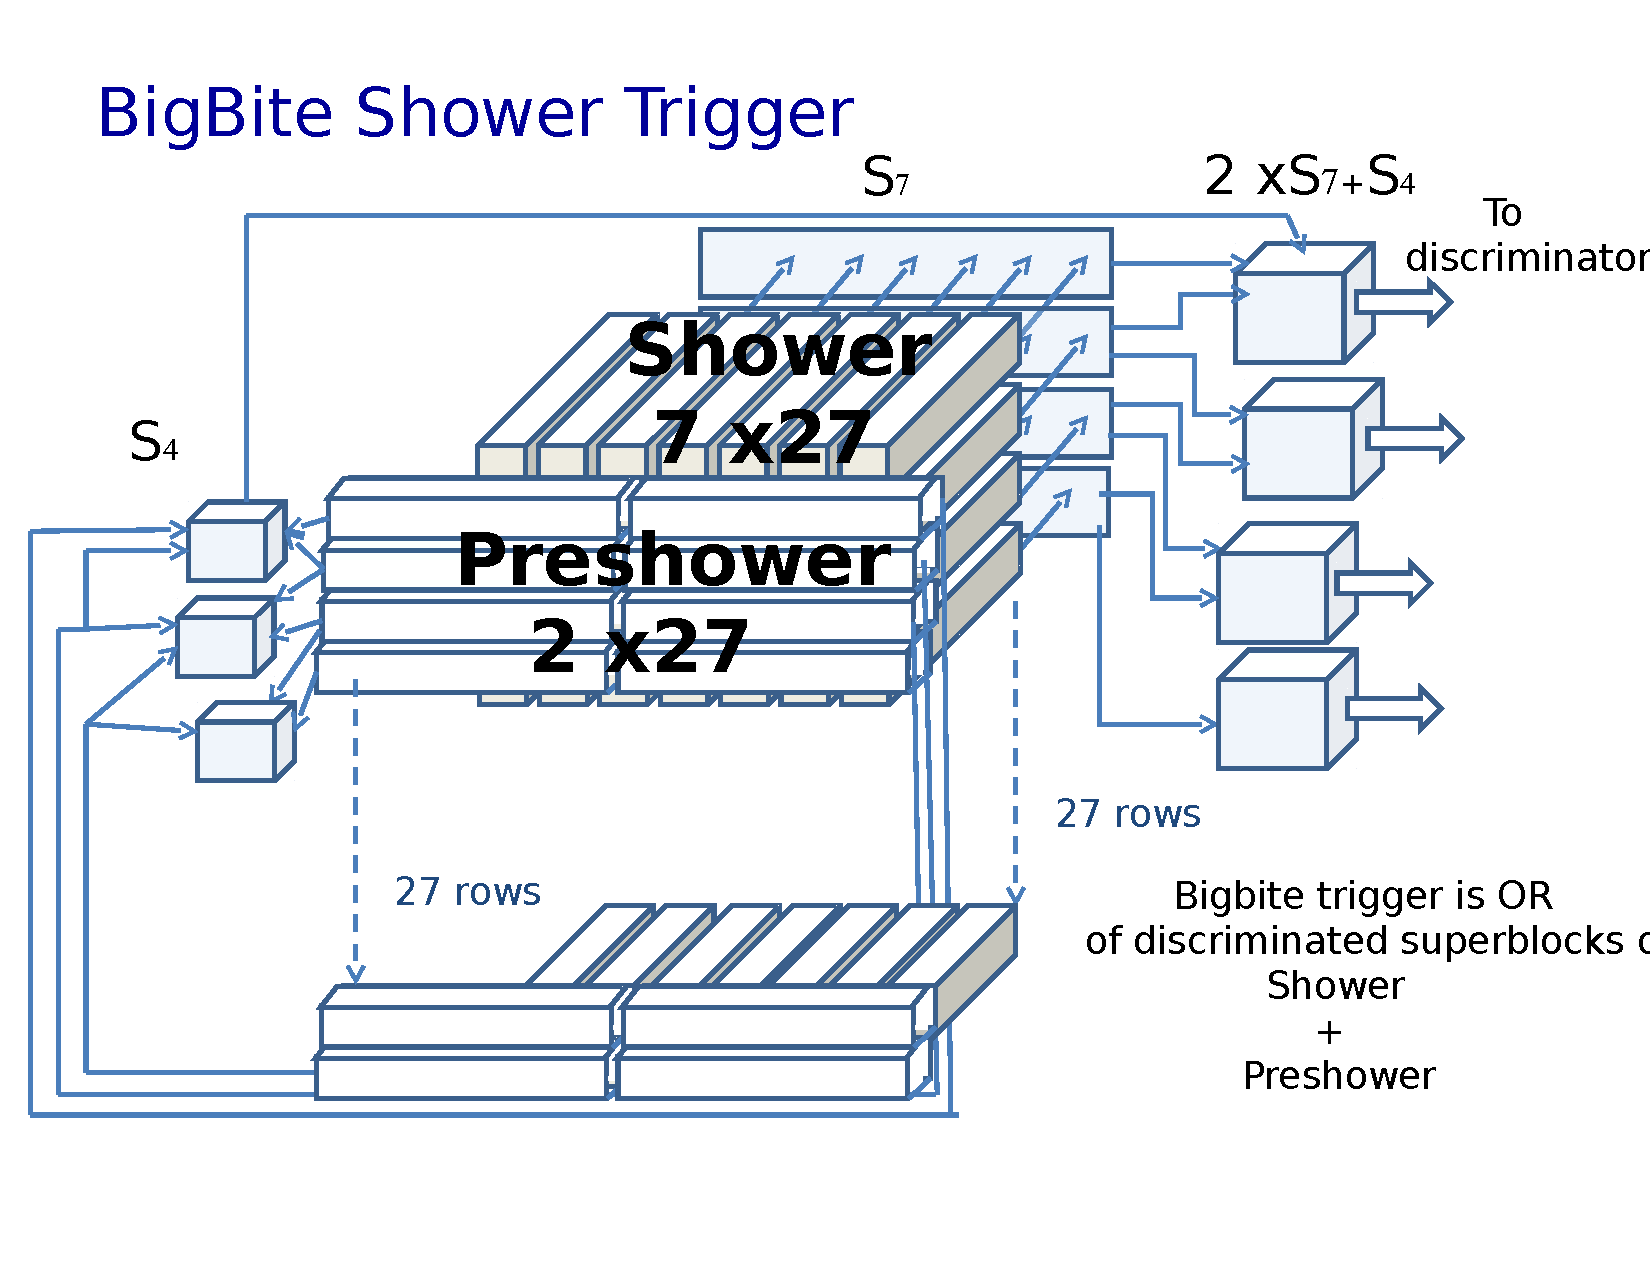
\includegraphics[width=0.8\textwidth]{figs/BBETrig3D.pdf}

\begin{table}
 	\begin{tabular}{|l|l|} \hline
 		Cable length from PMT to sum of 8 module & 57ns \\ \hline
 		Sum of 8 module transit time & 10ns \\ \hline
 		Cable from Sum of 8 module to FI/FO for group of 32 & 24ns \\ \hline
 		FI/FO module transit time & 10ns \\ \hline
 		Cable from FI/FO to the 16 channel discriminator & 4ns \\ \hline
 		 16 channel discriminator  transit time & 10ns \\ \hline
 		 Cable from the 16 channel discriminator to 16 channel mixed logic unit& 4ns \\ \hline
  		 16 channel mixed logic unit  transit time & 10ns \\ \hline
  		 Cable from the 16 channel mixed logic units to final 16 channel mixed logic unit& 4ns \\ \hline
  		 16 channel mixed logic unit  transit time & 10ns \\ \hline
  		 50M fast cable from the ECal platform to Trigger Supervisor & 200ns \\ \hline
  		 Transit time in TS to produce the ADC gate & 40ns \\ \hline
  		 Cable from TS to logic fan  & 6ns \\ \hline\hline
                 Logic fan  & 10ns \\ \hline\hline
                 Logic fan to FASTBUS crate & 25ns \\ \hline\hline
  		 Total time & 407 ns \\ \hline  		   		  		 		 
 	\end{tabular}
 	\caption{The contributions to total time formation of the ECal Level One trigger sued as the ADC gate.}
 	\label{tab:ECALTrigtime}
\end{table}

\subsection{GMn experiment}
\subsection {Expected trigger rates}
\begin{tabular}
  \hline
  \hline
  \hline
\end{tabular|

\subsection {Expected trigger rates}
 
%%\includegraphics[scale=0.55]{Gen_trig1.gif}\\
\subsection {Timing diagram}

\end{document}
